\chapter{Formal Security Analysis of Three Key Establishment Protocols}
\label{chp:analysis}


\section{Modelling Security Claims}

As mentioned in Section \ref{sec:attributes}, key establishment schemes desire certain security properties. In the verification of the security protocols of this thesis, the following properties are verified: \emph{Entity authentication}, \emph{Implicit key authentication}, \emph{Explicit key authentication}, \emph{Known-key secrecy}, \emph{Key control}, and \emph{Secrecy of key}. As mentioned in Section \ref{sec:attributes}, symmetric key establishment schemes are not resilient against \gls{kci} attacks, and do not provide forward secrecy. These properties are nevertheless included in the models as \gls{sakes} uses a lightweight version of public-key cryptography which is used to establish session keys.

\paragraph{Entity authentication:} Entity authentication between nodes corresponds to the security claim \texttt{Alive}, and can also be verified through stronger claims such as \texttt{Weakagree}. This property can only be violated if the adversary is able to inject or tamper with messages that are transmitted over the network, which we assume that the adversary in a \gls{6lowpan} network is.

\paragraph{Implicit key authentication} Implicit key authentication is modelled through the settings of the adversary compromise model described in Section \ref{sec:adversary}. The property is modelled by allowing the adversary to obtain the long-term keys and impersonate anyone except for the nodes that are supposedly establishing keys.

\paragraph{Explicit key authentication} Is achieved when the protocol satisfied both implicit key authentication and key confirmation. This is modelled through the security claim for \emph{non-injective agreement} denoted as \texttt{ni-agree}, but can also be modelled by using \texttt{running} and \texttt{commit} claims.

\paragraph{Known-key security} By revealing session keys to the adversary after usage (i.e. the session key is expired, and will never be used again) known-key security can be modelled. This is done by setting the \emph{Session-key reveal} rule in the adversary compromise model.

\paragraph{Key control} Scyther has no support for verifying key control. Therefore, this security property has to verified by hand. 

\paragraph{Secrecy of key} To model a key (or any other property) as secret, the \texttt{secrecy} claim is used in Scyther.

\paragraph{Forward secrecy} Both \gls{pfs} and \gls{wpfs} are related to active adversaries, and is modelled through the adversary compromise model, which can be configured to leak the long-term private key which the session keys are derived from.

\paragraph{Key compromise impersonation} \gls{kci} is also a property related to an active adversary, and is therefore available through the adversary model where the adversary can be allowed to obtain the long-term private key of the actors.


\section{Formal Security Analysis of APKES}

\gls{apkes} is modelled as two roles, the initiator $A$ and the responder $B$, agreeing upon a pairwise key through the message exchange that is presented in Figure \ref{fig:apkes-handshake}. There is not specified any concrete type of pluggable scheme (i.e. the scheme where \gls{apkes} obtains the shared secret between two nodes), hence we assume that whatever scheme is used is secure. In the model, the shared secret obtained from the pluggable scheme has been modelled using Scyther's built-in support for shared symmetric keys, where the two nodes $A$ and $B$ both possesses the shared secret at start-up.

\gls{apkes} states that the $R_A$ value has to be checked whether or not it has been tampered with, before the pairwise key can be derived at the initiating side. This can be verified by modelling the protocol to agree upon the $R_A$ value during the protocol execution, and committing to this. In addition, we model agreement over the pairwise key by using a \texttt{Running} claim in role $B$ after receiving the \texttt{ACK} authenticated with the pairwise key, and \texttt{Commit} claims in both roles to claim explicit key authentication on the pairwise key. As $B$ authenticates the $HELLOACK$ by using the shared secret, we do not claim that the pairwise key is created before $A$ receives the $HELLOACK$ from B. The Scyther model of \gls{apkes} can be viewed in its entirety in Appendix \ref{app:apkes}.

\subsection{Security Claims}

By taking starting point in the protocol specification from Section \ref{subsec:apkes-spec} and the alleged security properties from Section \ref{subsec:apkes-prop}, the protocol is modelled as an \gls{spdl}-script, which can be verified by Scyther. Listing \ref{lst:claims-a-apkes} describes the various security claims that is chosen for $A$. In these claims, we verify that the other party in the protocol is authentic, and that the pairwise key is secret. Claims for non-injective synchronization and agreement is also added to verify that the protocol executes as expected.

\begin{lstlisting}[caption={Security claims for role A in APKES.}, label={lst:claims-a-apkes}]
	claim(A, Alive);
	claim(A, Weakagree);
	claim(A, Niagree);
	claim(A, Nisynch);
	claim(A, Commit, B, Na);
	claim(A, Secret, PairwiseKey);
	claim(A, Commit, B, PairwiseKey);
\end{lstlisting}

In Listing \ref{lst:claims-b-apkes} below, the security claims for the role $B$ in \gls{apkes} are stated. Compared to the claims for $A$, $B$ does not contain the \texttt{Commit} claim, as the \texttt{Running}, \texttt{Commit} approach is used in role $A$ to provide agreement over the nonce $R_A$. We also claim non-injective synchronization and agreement.

\begin{lstlisting}[caption={Security claims for role B in APKES.}, label={lst:claims-b-apkes}]
	claim(B, Alive);
	claim(B, Weakagree);
	claim(B, Niagree);
	claim(B, Nisynch);
	claim(B, Secret, PairwiseKey);
	claim(B, Commit, A, PairwiseKey);
\end{lstlisting}


\subsection{Adversary}

In the description of \gls{apkes}, no specific adversary is mentioned. If we assume that such a protocol would be used for key establishment in \gls{6lowpan} networks, which are potentially deployed in hostile areas. Therefore, we can assume that the adversary would be able to observe, inject, and tamper with messages that are sent over the network. As \gls{apkes} does not utilize any session keys, but rather agreeing upon a fixed long-term key, we model the adversary in a Dolev-Yao way without giving it any active capabilities other than being able to obtain the long-term keys of nodes not participating in the current key establishment process. 

\subsection{Results}

Figure \ref{fig:apkes-verified} shows the verification result from running the model of \gls{apkes} through Scyther in the presence of the adversary described above. Scyther was able to perform an unbounded verification of the model where all claims but one were successfully verified. \gls{apkes} provides verifiable entity authentication, explicit key authentication for role $B$ (implicit for $A$), and holds the non-injective synchronization property, which means that every message in protocol is executed as expected, even in the presence of the adversary. When looking at the characterization of the protocol, there exist only one executable trace for each of the roles. Hence, there does not exist any malicious behaviour that can force the modelled protocol to misbehave. The attack proposed by Scyther on $Commit\ B, \{Na, Nb\}k(A,B)$ is not a direct attack on the protocol, but it shows that it is not possible to achieve explicit key authentication for the role $A$, as it has no knowledge of if $B$ has computed the pairwise key. 


\begin{figure}[h]
	\centering
	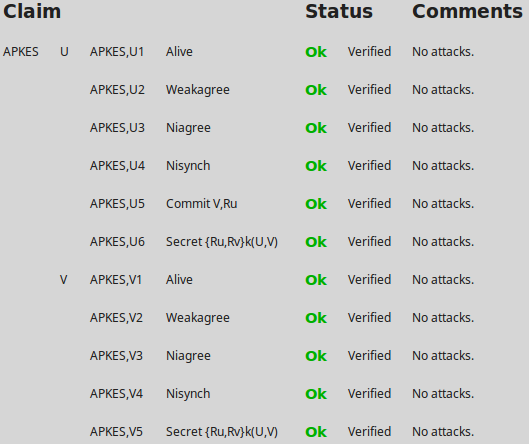
\includegraphics[scale=0.75]{analysis/apkes-verified.png}
	\caption{Result of verifying APKES' security claims using Scyther.}
	\label{fig:apkes-verified}
\end{figure}



\section{Formal Security Analysis of AKES}


\gls{akes} is modelled almost as its predecessor, but with additional content that is used to allow mobility for the devices. As \gls{akes} is used for establishing session keys, the \texttt{SKR} claim is used emphasize that the key is in fact a session key. The pluggable scheme is assumed to be secure, and is modelled as a symmetric key shared between the two communicating parties using Scyther's built-in symmetric key support. Appendix \ref{app:akes} contains the model in its entirety. 

\subsection{Security Claims}

From the protocol specification in Section \ref{subsec:akes-specs} and the assumed security properties in Section \ref{subsec:akes-props}, the following security claims are claimed to hold for the two roles in \gls{akes}, as seen in Listing \ref{lst:claims-a-akes} and Listing \ref{lst:claims-b-akes}. In addition to claiming authentication for the other party, we also claim that the protocol has been executed as intended by adding claims for non-injective synchronization and agreement. \gls{apkes} was not able to provide explicit key authentication of role $B$ for the initiator $A$. In \gls{akes}, however, the received \texttt{HELLOACK} is authenticated using the session key. Therefore, we model a \texttt{Running} claim 

\begin{lstlisting}[caption={Security claims for role A in AKES.}, label={lst:claims-a-akes}]
	claim(A, SKR, SessionKey);
	claim(A, Alive);
	claim(A, Weakagree);
	claim(A, Niagree);
	claim(A, Nisynch);
	claim(A, Commit, B, SessionKey);
\end{lstlisting}

\begin{lstlisting}[caption={Security claims for role B in AKES.}, label={lst:claims-b-akes}]
	claim(B, SKR, SessionKey);
	claim(B, Alive);
	claim(B, Weakagree);
	claim(B, Niagree);
	claim(B, Nisynch);
	claim(B, Commit, A, SessionKey);
\end{lstlisting}

\subsection{Adversary}

The adversary in this model is nearly the same adversary as the one introduced in the verification of \gls{apkes}. However, to model session keys, the adversary is allowed to obtain all session keys whose identifier differs from the current protocol execution. 
\newpage
\subsection{Results}

Figure \ref{fig:akes-verified} shows the result of running the model of \gls{akes} through Scyther in the presence of the adversary presented above. \gls{akes} is verified for an unbounded state space with all the claimed security properties successfully verified. \gls{akes} provides provable authentication for the roles, as well as explicit key authentication for both parties. In addition, \gls{akes} is proved to hold the non-injective synchronization claim which states that the protocol was executed as intended. When looking at the characterization of \gls{akes} only one possible trace is returned for each role, which means that there exists only one way to execute the protocol.

\begin{figure}[h]
	\centering
	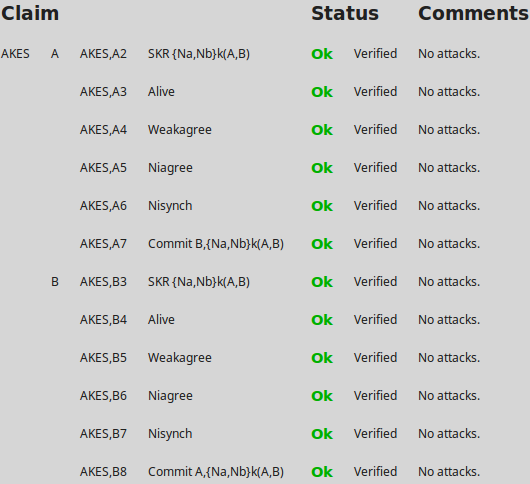
\includegraphics[scale=0.95]{analysis/akes-verified.png}
	\caption{Result of verifying AKES' security claims using Scyther.}
	\label{fig:akes-verified}
\end{figure}


\section{Formal Security Analysis of SAKES}
\label{sec:anal-sakes}

From the protocol specification in Section \ref{subsec:sakes-spec} and the assumed security properties in Section \ref{subsec:sakes-props} \gls{sakes} have been modelled into four roles $A$ (End device), $B$ (Router), $C$ (Border router), and $D$ (Server). The authentication phase is carried out between $A$, $B$, and $C$, before $B$ and $D$ establishes the session key. As the protocol specification presented in the original protocol proposal can be considered inconsistent, some assumptions have been made in the model. For starters, it is assumed that the Diffie-Hellman key agreement is completed correctly by letting $B$ and $D$ share their secret key to the power of the generator $g$. In addition, it is also assumed that when the authors use notion of ``decrypting the ciphertext encrypted with the private key of $X$'', they actually mean that the message is signed using the private key of $X$, and that the signature can be verified by applying the corresponding public key. When it comes to the notation of \gls{mac-auth}s, an assumption is that the alleged \gls{mac-auth} that is sent between the router and the server that do not share any symmetric key is simply a hash of the message. 

As \gls{sakes} uses Diffie-Hellman, which Scyther does not originally support, a ``hack'' have been introduced to model that it is not possible for the adversary to compute the session key by possessing either one of the two secret keys that are used in the computation. This can be modelled by introducing a helper protocol in Scyther that underapproximates $g^{x}$ into $hashfunction(g, x)$. The helper protocol is shown in Listing \ref{lst:helper} and is marked with the at-symbol (@). This states that the two terms $g2(g1(T1),T2)$ and $g2(g1(T2), T1)$ are approximate equal.

\begin{lstlisting}[caption={Helper protocol to model Diffie-Hellman in SAKES.}, label={lst:helper}]
hashfunction g1, g2;

protocol @exponentiation(DH)
{
	role DH
	{
		var T1,T2: Ticket;

		recv_!1(DH, DH, g2(g1(T1),T2) );
		send_!2(DH, DH, g2(g1(T2),T1) );
	}
}
\end{lstlisting}

\subsection{Security Claims}

The end device $A$ is only in direct communication with the router $B$ and the border router $C$, which is why authentication is only claimed for these two roles as seen in Listing \ref{lst:claims-a-sakes}. We also claim that the generated session key should be secret by using the \texttt{SKR} claim. 

\begin{lstlisting}[caption={Security claims for role A in SAKES.}, label={lst:claims-a-sakes}]
		claim_A1(A, Alive, B);
		claim_A2(A, Alive, C);
		claim_A3(A, Weakagree, B);
		claim_A4(A, Weakagree, C);
		claim_A5(A, Niagree);
		claim_A6(A, Nisynch);
		claim_A7(A, SKR, SessionKeyA);
\end{lstlisting}


Listing \ref{lst:claims-b-sakes} contains the claims that are stated for role $C$ in \gls{sakes}, which is the \gls{6lowpan} router. The router is interacting with all the other entities in the network, and hence we are claiming authentication for each of these roles. In addition, we state that the ephemeral key $Sk_B$ which is generated by the border router during the authentication phase and used in the key establishment, is secret. In addition, we add claims for non-injective synchronization and agreement to ensure that the protocol behaves as intended.

\begin{lstlisting}[caption={Security claims for role B in SAKES.}, label={lst:claims-b-sakes}]
		claim_B1(B, Secret, Sk);
		claim_B2(B, Alive, A);
		claim_B3(B, Alive, C);
		claim_B4(B, Alive, D);
		claim_B5(B, Weakagree, A);
		claim_B6(B, Weakagree, C);
		claim_B7(B, Weakagree, D);
		claim_B8(B, Niagree);
		claim_B9(B, Nisynch);
\end{lstlisting}

The border router $C$ does only communicate with the end device and the router, hence we do only claim authentication for these two parties. In addition we add claims for non-injective synchronization and agreement to state that the protocol was executed as expected as seen in Listing \ref{lst:claims-c-sakes}. 

\begin{lstlisting}[caption={Security claims for role C in SAKES.}, label={lst:claims-c-sakes}]
		claim_C1(C, Alive, A);
		claim_C2(C, Alive, B);
		claim_C3(C, Weakagree, A);
		claim_C4(C, Weakagree, B);
		claim_C5(C, Niagree);
		claim_C6(C, Nisynch);
\end{lstlisting}

For the remote server, authentication is claimed only between it and the router which is establishes session keys with. The end device is indirectly authenticated through the proof that is signed by the authentication module in the border router, but this is not modelled as a direct authentication claim in this model. The generated session key $Sk_D$ is claimed to be secret using the \texttt{SKR} notation. In addition, we also claim non-injective synchronization and agreement for the role as seen in Listing \ref{lst:claims-d-sakes}.


% run verification with Alive, Weakagree, for A?
\begin{lstlisting}[caption={Security claims for role D in SAKES.}, label={lst:claims-d-sakes}]
		claim(D, Alive, B);
		claim(D, Weakagree, B);
		claim(D, Niagree);
		claim(D, Nisynch);
		claim(D, SKR, SessionKeyD);
\end{lstlisting}

\subsection{Adversary}

For \gls{sakes} we assume a Dolev-Yao adversary which is capable of eavesdropping, delete messages, compute cryptographic analysis on intercepted messages, forge new messages from its knowledge, and insert them into the network. It is allowed for the adversary to obtain the session keys for all sessions whose identifier differs from the current session identity. As \gls{sakes} utilizes a form of Diffie-Hellman key agreement, it is also assumed that the protocol should possess forward secrecy, especially since the half of the key is fixed as the remote server uses a permanent public key pair.

\subsection{Results}

The results of verifying the model of \gls{sakes} using Scyther is presented in Figure \ref{fig:sakes-verified}. As we see, multiple of the security properties that should be claimed for \gls{sakes} are falsified by Scyther. When looking at the characterization of \gls{sakes}, more than 96 traces are found for the different roles, which might indicate that the protocol is poorly designed. As it is difficult for a human being to identify possible error states as the state space increases, it is fair to assume that the possibility of possible attacks increases with the number of traces. The verification was conducted with an upper bound of five runs, where the \texttt{ok} status indicates that no attack was found within this bound. Increasing the upper bound was experimented with. However, as the verification of the original protocol and an upper bound of five runs took approximate 10 hours to complete on a workstation with an Intel Core i7 processor and 12 GB \gls{ram}, the experiment was quickly abandoned.

\subsubsection{A - End Device}

For the end device, the only security properties that are successfully verified are entity authentication for the router $B$ and secrecy for the computed session key. \gls{sakes} is not able to provide stronger authentication for the router, nor any authentication at all of the border router $C$. Also, the claims for non-injective synchronization and agreement does not hold for the end device.

\subsubsection{B - Router}

The router is able to provide entity authentication for all other roles within in the bound, and could also provide stronger authentication such as \texttt{Weakagree} for the end device and the border router. This is because of the use of cryptographic nonces and \gls{mac-auth}s that are generated using the secret symmetric keys that are shared between the entities. \gls{sakes} does not, however, provide non-injective synchronization and agreement. One can argue that this is because of the inconsistency of the protocol, and that the key establishment process overlooks some authentication properties as it solely relies on the proof that is signed and delivered by the border router and the ephemeral key pair. 

\subsubsection{C - Border Router}

As with the end device and the router, the border router $C$ is also able to provide entity authentication for $A$ and $B$. It does not, however, provide non-injective synchronization or agreement. The border router only communicates with $A$ and $B$.



\subsubsection{D - Remote Server}

\begin{figure}[h]
	\centering
	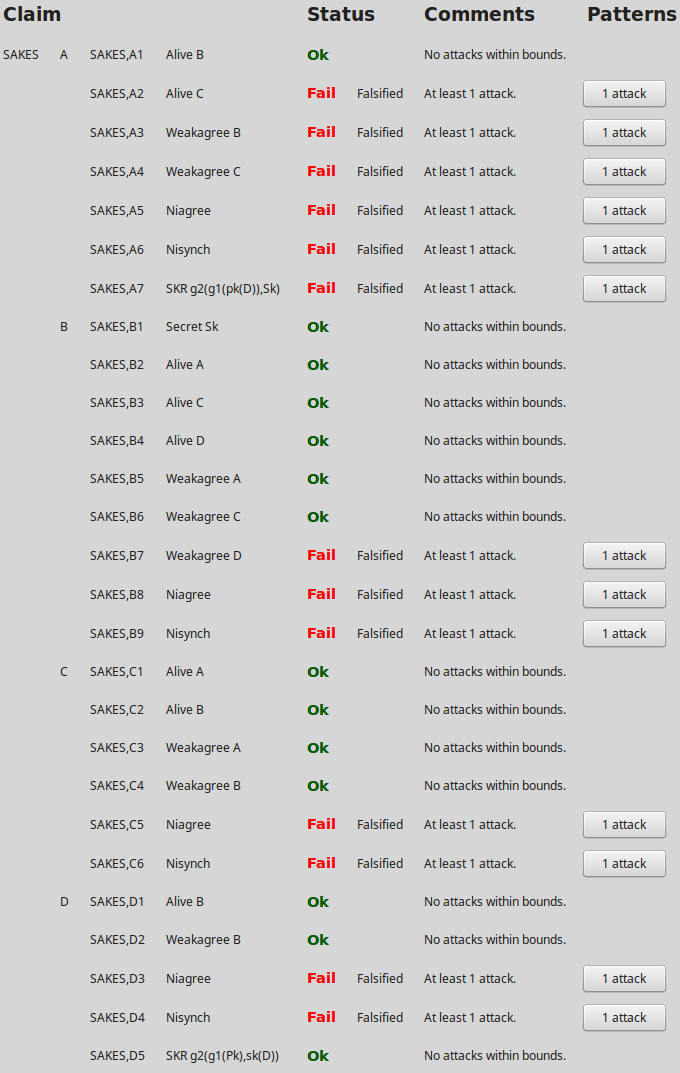
\includegraphics[scale=0.70]{analysis/sakes-verified-dy.png}
	\caption{Result of verifying SAKES' security claims using Scyther.}
	\label{fig:sakes-verified}
\end{figure}





% How to check for properties:

% Forward Secrecy: Not able to achieve in symmetric key. Check through Scyther rules.

% Known-Key Security: Session-Key reveal

% Key Confirmation: running, commit / niagree

% Key Compromise Impersonation: Impossible to achieve in protocols relying on symmetric keys? Need asymmetric? Boyd book. SKR claim of an entity whose long-term key is revealed to the adversary

% Unknown key share: Known-Key Security?

% Entity authentication: From A to B: Aliveness of A in B's claims.

% Implicit: Long-term reveal for other entities than A and B.

% Explicit. Implicit + key confirmation
